\subsection{Deleting vs. removing elements from diagrams} 

A central feature that new users should understand as soon as possible is the way EA handles diagrams. A diagram is simply treated as a \emph{view} of the
complete ``model'' in EA. The complete model can always be browed in a tree view (the package browser) and contains all elements that are exported. Diagrams
typically do not contain all elements and one usually uses multiple possibly ``redundant" diagrams to show different parts of the model. Thinking in this frame
is crucial and provides a pragmatic solution to the problem of having huge unmaintainable diagrams. A tricky consequence one must get used to is that
\emph{removing} an element from a diagram does \emph{not} delete it from the model.

\begin{enumerate}
\item[$\blacktriangleright$] One of the most common mistakes of new users is to remove an element from a diagram by pressing \texttt{Del} and expecting the
element to be deleted from the model.
This is however not the case as the element is only removed from the current diagram and is still in the model and thus in the package browser
(Fig.~\ref{fig_DelVsCtrlDel01}).

\begin{figure}[htbp]
\begin{center} 
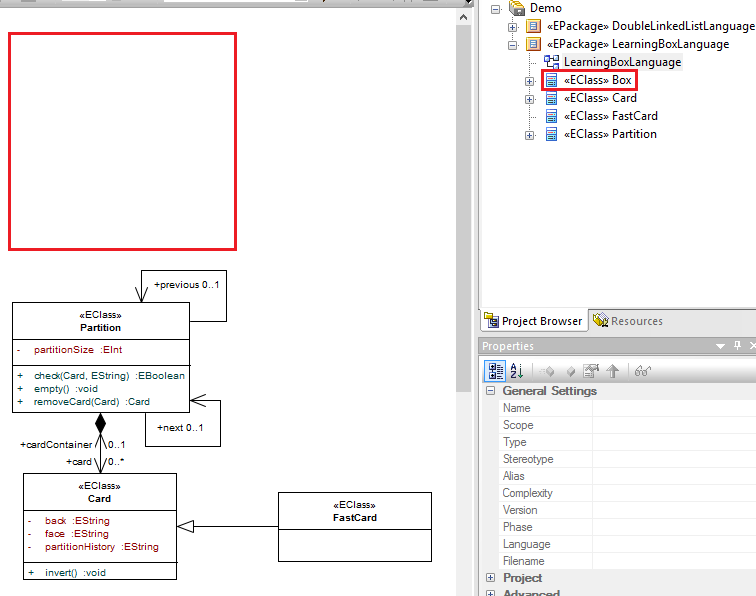
\includegraphics[width=0.87\textwidth]{DelVsCtrlDel1}
  \caption{Removing an element from a diagram via pressing \texttt{Del} does not delete it from the model and it is still present in the package browser}  
    \label{fig_DelVsCtrlDel01}
\end{center}
\end{figure}  

\item[$\blacktriangleright$] By pressing \texttt{Ctrl+Del} and confirming (Fig.~\ref{fig_DelVsCtrlDel02}) you can \emph{delete} an element from a diagram
\emph{and} completely from the model as well (the element will no longer be in the \texttt{Project Browser}). Elements can also be deleted via the context menu
in the \texttt{Project Browser} (invoked by right-clicking the element in the \texttt{Project Browser}).

\begin{figure}[htbp]
\begin{center}
  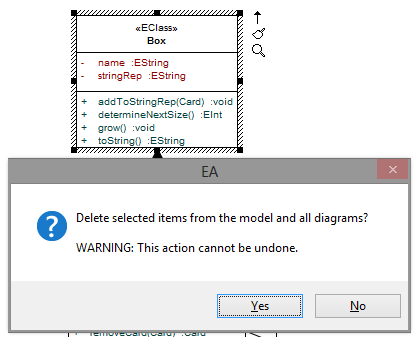
\includegraphics[width=0.7\textwidth]{DelVsCtrlDel2}
  \caption{Deleting an element from a diagram and from the model}  
  \label{fig_DelVsCtrlDel02}
\end{center}
\end{figure}  

\end{enumerate}